%
% TODO
% Sashank's and Nakayama's environmental, repair transitions and numerical optimizations (U/D states).
% Talk about environment dependent phis in Remarks?
% Cache for BFH Eval
%

\documentclass[12pt]{article}
\author{M. Sanghavi, S. Tadepalli, M. Nakayama}
\date{January 2013}

\usepackage{graphicx}
\usepackage{algorithm}
\usepackage{algorithmic}
\usepackage{mathabx}
\usepackage[left = 1.0in, top = 1in, right = 1.0in, bottom = 1in, nohead]{geometry}

\newcommand{\captionAmerica}[2]{
\noindent\hspace{\fill}\rule{1.0\linewidth}{.7pt}\hspace{\fill}\vspace{-0.25em}\\*\raggedright\textbf{Algorithm #1} #2 \vspace{-0.8em}\\*\hspace{\fill}\rule{1.0\linewidth}{.7pt}\hspace{\fill}
}
\newcommand{\varName}[1]{\textrm{\it#1}}
\newcommand{\citeLine}[1]{$\{\,#1\,\}$}
\newcommand{\citeBlock}[2]{$\{\,#1 - #2\,\}$}

\begin{document}
\title{Working Title}
\maketitle

% \section{Introduction}

% \section{Model}

\section{Model}
\label{sec:model}

We work with the stochastic model
of \cite{ING:2009}, which considers
the evolution over time
of a repairable dependability system
operating in a randomly changing environment.
The system consists of
a collection
$\Omega = \{ 1, 2, \ldots, N \}$
of $N < \infty$ component types.
Each component type~$i \in \Omega$
has a redundancy $1 \leq r_i < \infty$,
and the $r_i$ components of type~$i$
are assumed to be identical.
A component can be either
operational (up) or failed (down).

The environment changes randomly
within a set
$\mathcal{E} = \{ 0, 1, 2, \ldots, L \}$.
For example, we can think of the environment
as representing the current load on the system,
and if there are two possible environments,
$0$ and $1$, then $0$ (resp., $1$)
may represent a low (resp., high) load.
Once the environment enters $e \in \mathcal{E}$,
it remains there for an exponentially distributed
amount of time with rate $\nu_e > 0$,
after which the environment changes
to $e'$ with probability $\delta_{e,e'}
\geq 0$,
where $\delta_{e,e} = 0$
and $\sum_{e' \in \mathcal{E}} \delta_{e,e'} = 1$.
We assume the matrix $\delta = (\delta_{e,e'} :
e, e' \in \mathcal{E})$ is irreducible;
i.e.,
for each $e, e' \in \mathcal{E}$,
there exists $k \geq 1$ and a sequence
$e_0 = e, e_1, e_2, \ldots, e_k = e'$
with each $e_i \in \mathcal{E}$ such that
$\prod_{i=0}^{k-1} \delta_{e_i, e_{i+1}} > 0$.
In other words, it is possible to eventually
move from environment $e$ to
environment $e'$.

The components in the system can randomly
fail and then be repaired.
When the environment is $e \in \mathcal{E}$,
the failure rate and repair rate
of each
component of type $i$
are $\lambda_{i,e} > 0$ and $\mu_{i,e} > 0$,
respectively.  If there is only one
environment $e$, i.e., $| \mathcal{E} | = 1$,
then the lifetimes and repair times of
components of type $i$ are exponentially
distributed with rates $\lambda_{i,e}$
and $\mu_{i,e}$, respectively.
Exponential distributions are
frequently used to model
lifetimes of hardware and
software components; e.g.,
see \cite{XDP:2004}.
We assume that all operating components
of a type~$i$ have the same failure
rate $\lambda_{i,e}$ in environment $e$.
Thus, in a system with  redundancies
for which not all components of a type
are needed for operation of the system,
the extras are ``hot spares'' since
they fail at the same rate as the main
components.

Our model includes probabilistic
instantaneous cascading failures,
which occur as follows.
The ordered set $\Gamma_i$ specifies
the types of components
that a failure of a type-$i$ component
can cause to simultaneously fail.
When a component of type $i$ fails,
it causes a single 
component of type~$j \in \Gamma_i$
to fail at the same time
with probability
$\phi_{i,j}$
(if there are components of type $j$ up).
The events that the individual components
types~$j \in \Gamma_i$
fail immediately are independent.
Thus, when a component of type $i$ fails,
there are independent ``coin flips''
to determine which components in $\Gamma_i$ fail,
where the coin flip for $j \in \Gamma_i$
comes up heads (one component of
type $j$ fails) with probability $\phi_{i,j}$
and tails
(no components of type $j$ fail)
with probability $1 - \phi_{i,j}$.

We allow for a cascading failure to continue
as long as there are still components operational
in the system.  For example, the failure of
a component of type $i$ may cause
a component of type $j$ to fail
(with probability $\phi_{i,j}$),
which in turn causes a component of type $k$
to fail (with probability $\phi_{j,k}$),
and so on.
As noted in \cite{ING:2009},
the SAVE package \cite{BHLNS:1994}
allows for only one level of cascading,
but the unlimited cascading in our model
makes it significantly more difficult
to analyze.

We can think of a cascading failure
as a tree of simultaneously failing components.
The root is the component, say of type $i$,
whose failure \textit{triggers} the cascade.
The root's children, which are from
$\Gamma_i$, are those components
whose immediate failures
were directly caused by the
root's failure.
At any non-root level of the tree, 
these components'
failures were directly caused by the
failure of their parents at the previous level.
Although all the failing components
in a cascade fail at the same time,
we need to specify an order in which
they fail for our problem to
be well-defined, as we explain later.
We assume the components in a tree
fail in breadth-first order.


There is a single repairman who
fixes failed components using
a processor-sharing discipline.
Specifically, if the current
environment is $e$ and there
is only one failed component,
which is of type~$i$, then
the repairman fixes that component
at rate $\mu_{i,e}$.
If there are $b$ components currently failed,
then the repairman allocates $1/b$ of
his effort to each failed component,
so a failed component of type $i$ is
repaired at rate $\mu_{i,e}/b$.



\section{Markov Chain}
\label{sec:ctmc}


We want to analyze the behavior of the
system as it evolves over time.  Because of the
processor-sharing repair discipline
and the exponential distributions
for the event lifetimes,
it will suffice to define the
state of the system as a vector
containing
the
number of failed components of each type
and
the current environment.
Thus, let
$S = \{ x = (x_1, x_2, \ldots, x_N, x_{N+1}) :
0 \leq x_i \leq r_i \ \forall i \in \Omega, \,
x_{N+1} \in \mathcal{E}
 \}$
be the state space,
and let $Z = [Z(t) : t \geq 0]$
be the continuous-time Markov time (CTMC)
living on $S$ keeping track
of the current state of the system.
(If we had instead considered
a first-come-first-served repair
discipline, then the state
space would need to be augmented to
keep track of the order in which
current set of down components failed.)

We assume that $Z$ starts in
environment $0 \in \mathcal{E}$
with no
components failed, i.e., state
$(0,0, \ldots, 0)$, and we
now describe the CTMC's infinitesimal
generator matrix $Q = (Q(x,y) : x, y \in S)$,
where $Q(x,y)$ is the rate that
the CTMC $Z$ moves from state
$x = (x_1, \ldots, x_N, x_{N+1})$
to state $y = (y_1, \ldots, y_N, y_{N+1})$.
If
$y_i = x_i$ for each $i \in \Omega$
and
$y_{N+1} \neq x_{N+1}$,
then
$(x,y)$ is an \textit{environment transition}
with $Q(x,y) = \nu_{x_{N+1}} \delta_{x_{N+1},y_{N+1}}$.
If
$y_i = x_i - 1$ for one $i \in \Omega$,
$y_j = x_j$ for each $j \in \Omega - \{ i \}$,
and
$y_{N+1} = x_{N+1}$,
then $(x,y)$
is a \textit{repair transition}
corresponding to the repair
of a component of type $i$,
and
$Q(x,y) =
x_i \mu_{i,x_{N+1}}/(\sum_{j \in \Omega} x_j)$.
If
$y_i \geq x_i$ for all $i \in \Omega$
with $y_j > x_j$ for some $j \in \Omega$
and
$y_{N+1} = x_{N+1}$,
then $(x,y)$ is a
\textit{failure transition}
in which $y_i - x_i$ components
of type~$i$ fail, $i \in \Omega$.
Any other $(x,y)$ with $x \neq y$
not falling
into one of the above three categories
is not possible, so $Q(x,y) = 0$.
The diagonal entry $Q(x,x)
= -\sum_{y \neq x} Q(x,y)$,
as required for a CTMC.\@

We now determine the rate $Q(x,y)$ of
a failure transition $(x,y)$.
First consider the case when there is
no cascading failures possible,
i.e.,
$\Gamma_i = \emptyset$ for each type~$i$.
Then the only possible failure transitions
$(x,y)$ have
$y_i = x_i + 1$ for one $i \in \Omega$,
$y_j = x_j$ for each $j \in \Omega - \{ i \}$,
and
$y_{N+1} = x_{N+1}$,
and this corresponds to a single
component
of type~$i$ failing.
Then $Q(x,y) = (r_i - x_i)
\lambda_{i,x_{N+1}}$.

Cascading failures complicate the
computation of $Q(x,y)$
for a failure transition $(x,y)$.
As mentioned before, a cascading
failure is modeled as a tree $T$
built from the multiset $B$ of 
simultaneously failing
components,
where $B$ has
$y_\ell - x_\ell$ failing components
of type $\ell$, $\ell \in \Omega$.
A tree $T$ has a rate $R(T)$ determined
by the failure rate
$(r_i - x_i) \lambda_{i,x_{N+1}}$
of the root (assumed here to be of type $i$),
as well as the product of $\phi_{j,k}$
for a parent node of type $j$ causing
a child of type $k \in \Gamma_j$ to fail,
and $1 - \phi_{j,k}$ from
a node of type $j$
\textit{not} causing
a component of type $k \in \Gamma_j$
to fail when there are
components of type $k$ up.
A difficulty arises since
there can be many such trees
corresponding to the multiset $B$
of components failing in $(x,y)$,
and determining $Q(x,y)$ requires
summing $R(T)$ over all possible
trees $T$ that can be constructed
from $B$.
The number of such trees
grows exponentially in the
number of failing components in the
cascade; see \cite{ING:2009}.


\textbf{[The following is not complete
and will need to be changed
for another example.]}
Computing the rate $R(T)$ of a tree $T$
requires that the components fail
in a certain order, even though all
of the failures occur simultaneously.
To see why, consider the following example.
Let $\Omega = \{ A, B, C \}$,
with $r_A = r_B = r_C = 4$.
Also, let
$\Gamma_A = \{ B, C \}$,
$\Gamma_B = \{ A, C \}$,
and
$\Gamma_C = \{ A, B \}$.
Suppose that $\mathcal{E} = \{ 0 \}$,
and consider the failure transition
$(x,y)$ with
$x = (2, 2, 2, 0)$
and
$y = (4, 4, 3, 0)$.
Thus, $(x,y)$ corresponds
to $2$ components each of
types $A$ and $B$ failing
and a single component of type
$C$ failing.
One possible tree $T$
corresponding to $(x,y)$
is shown in Figure~\ref{fig:tree}.



\begin{figure}
\begin{center}
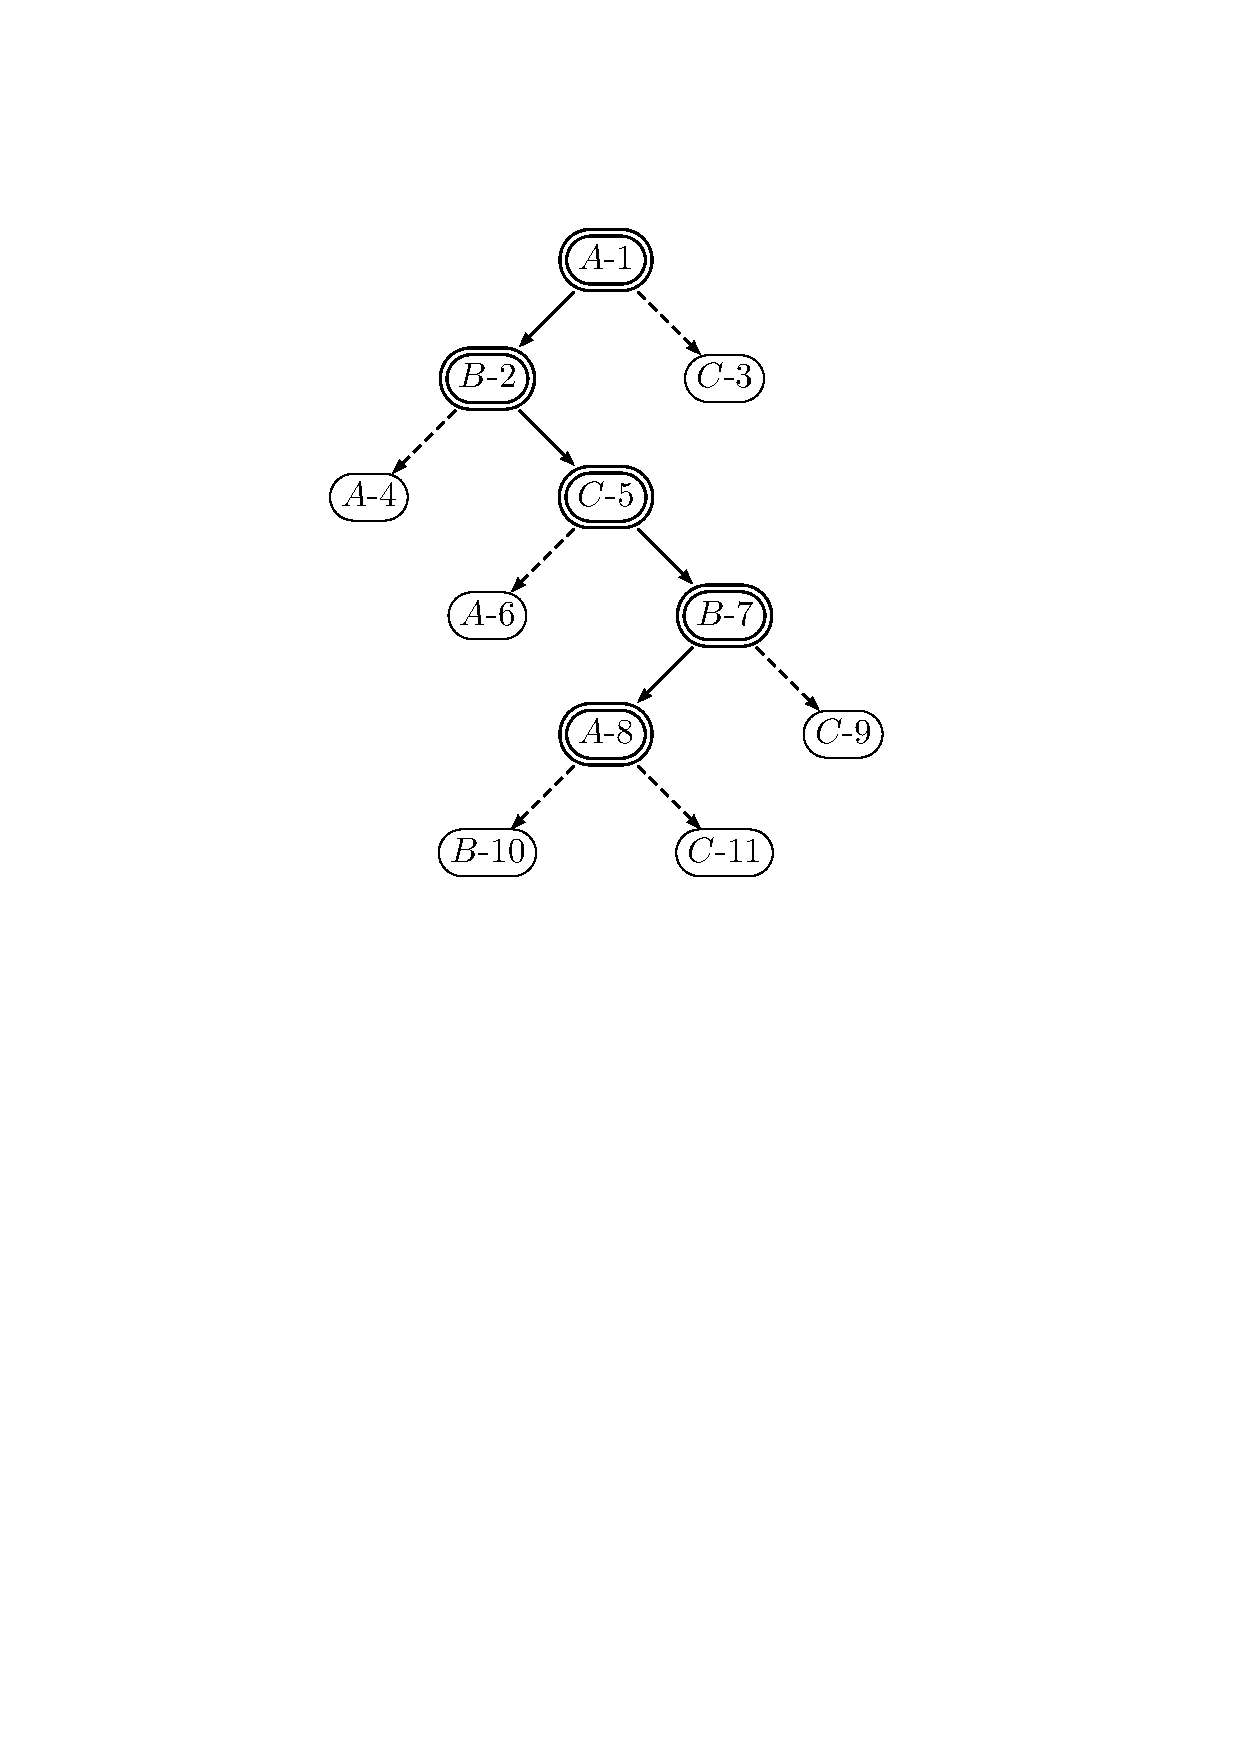
\includegraphics[width=0.4\textwidth]{fig_tree}
\end{center}
\caption{An example of a supertree.}
\label{fig:tree}
\end{figure}


The nodes depicted as double circles
form the tree of failing components.
The single circles correspond to
components in some $\Gamma_i$ set
but did not fail.  A component type
$j$ in some $\Gamma_j$ could have
not failed because there are
components of type $j$ up at this
point but its coin flip
came up tails 
(with probability $1 - \phi_{i,j}$),
or there were no more components of
type $j$ up at this point.
Each node has a label of the form
$t$-$i$, where $t$ denotes the
type of the component for that node,
and $i$ is the ID, which
is the position of the node
in a breadth-first ordering of
all the nodes (single and double circles).
We include the IDs just to simplify
the discussion here.
We call the tree of all nodes
the \textit{supertree} corresponding
to the tree $T$ of failing nodes.
The supertree is used to compute
the rate $R(T)$ of $T$, as follows.
Since the root is a component of
type~$A$ and there are
$r_A - x_A = 2$ components of type~$A$
at the start of the transition $(x,y)$,
the rate of the trigger of the cascade
is $2 \lambda_{A,0}$.
The root then causes a component
of type $B$ to fail at node ID $2$,
and this occurs with probability
$\phi_{A,B}$.
The node at ID $3$ did not fail,
and at this point there are
$r_C - x_C = 2 > 0$ components of type $C$
still up, so this nonfailure occurs
with probability $1 - \phi_{A,C}$.


\bibliographystyle{ieeetr}
\bibliography{mkn}
\end{document}